\begin{frame}{Evaluation}{Etat des lieux}
    \begin{itemize}[<+->]
        \item<1-> Traditionnelle

        \visible<3->{
            \begin{itemize}[<+->]
                \item Via une assignation
            \end{itemize}
        }

        \item<2-> Paresseuse

        \visible<4->{
            \begin{itemize}[<+->]
                \item Via un \texttt{callback}
            \end{itemize}
        }
    \end{itemize}
\end{frame}

\begin{frame}[fragile]{Evaluation traditionnelle}{Un exemple}
    \begin{lstlisting}[firstnumber=1]
        <?php

        $var = 'foobar';
    \end{lstlisting}
\end{frame}

\begin{frame}[fragile]{Evaluation traditionnelle}{Un autre exemple}
    \begin{lstlisting}[firstnumber=1]
        <?php

        $var = range(0, 1000 ** 3);
    \end{lstlisting}
\end{frame}

\begin{frame}[fragile]{Evaluation traditionnelle}{Un autre exemple\ldots oops!}
    \begin{spverbatim}
        PHP Fatal error: Allowed memory size of 536870912 bytes exhausted (tried to allocate 34359738376 bytes) in example.php on line 5
    \end{spverbatim}
\end{frame}

\begin{frame}[fragile]{Evaluation paresseuse}{Un autre exemple\ldots une solution?}
    \begin{lstlisting}[firstnumber=1]
        <?php

        $callback = static fn(): array => range(0, 1000 ** 3);
    \end{lstlisting}
\end{frame}

\begin{frame}{Evaluation paresseuse}{Un \textit{thunk}, définition}
    \begin{itemize}[<+->]
        \item Un \textit{thunk} est un \colorbox{yellow}{\textbf{conteneur}}
        \item Un \textit{thunk} est un \texttt{callback} avec une
        \colorbox{yellow}{\textbf{\textit{plus-value}}} sémantique en terme de
        précision.
        \item Un \textit{thunk} est l'expression d'une valeur qui est en
        \colorbox{yellow}{\textbf{attente d'evaluation}}.
        \item Un \textit{thunk} est une function qui enrobe (\texttt{wrap}) une
        expression, pour \colorbox{yellow}{\textbf{postposer}} son evaluation.
        \item L'origine du terme est né comme une version humoristique du passé
        du verbe anglophone \textit{penser} (\textit{to think}).
    \end{itemize}
\end{frame}

\begin{frame}[fragile]{Evaluation paresseuse}{Via un \texttt{callback} ou \textit{thunk}}
    \begin{lstlisting}[firstnumber=1]
        <?php

        $callback = static fn(): array => range(0, 1000 ** 3);

        $callback();
    \end{lstlisting}
\end{frame}

\begin{frame}[fragile]{Evaluation paresseuse}{Coïncidence?? Je ne crois pas!}
    \begin{spverbatim}
        PHP Fatal error: Allowed memory size of 536870912 bytes exhausted (tried to allocate 34359738376 bytes) in example.php on line 5
    \end{spverbatim}
\end{frame}

\begin{frame}[fragile]{Evaluation paresseuse}{Via un \texttt{callback} ou \textit{thunk}}
    
\includegraphics[width=\textwidth]{meme/wtf.png}
\end{frame}

\begin{frameC}{On récapitule\ldots}

\end{frameC}

\begin{frame}{Evaluation paresseuse}{Les \textit{thunk}, récap}
    \begin{itemize}[<+->]
        \item Un \textit{thunk} est un \colorbox{yellow}{\textbf{callable}} qui fait office de \colorbox{yellow}{\textbf{conteneur}}

        \item Utile pour \colorbox{yellow}{\textbf{retarder}} l'exécution d'un morceau de code

        \item Pratique pour les données \colorbox{yellow}{\textbf{scalaires}}

        \item N'est pas la solution magique à tous les problèmes
    \end{itemize}
\end{frame}

\begin{frameC}{Et pour les collections alors ?}

\end{frameC}

\begin{frame}{Evaluation paresseuse}{Etat des lieux}
    Existe t'il un moyen de faire une \colorbox{yellow}{\textbf{évaluation paresseuse}} sur un \colorbox{yellow}{\textbf{ensemble de
    données}} ?

    \pause
    \bigskip

    Une sorte de \textit{thunk}, qui pourrait \colorbox{yellow}{\textbf{itérer}}
    sur les élements d'une collection et renvoyer ces élements
    \colorbox{yellow}{\textbf{un par un}}, sans jamais renvoyer/évaluer le
    résultat dans sa globalité.
\end{frame}

\begin{frameC}{Oui, ça existe!}

\end{frameC}

\begin{frame}{Evaluation paresseuse}{Les itérateurs}
    \begin{itemize}[<+->]
        \item Les itérateurs
        \item Les générateurs
    \end{itemize}
\end{frame}

\begin{frame}[fragile]{Evaluation paresseuse}{Via un itérateur}
    \begin{lstlisting}[firstnumber=1]
        <?php

        // Evaluation traditionnelle
        foreach (range(0, 1000 ** 3) as $value) {
            // FATAL ERROR
        }
    \end{lstlisting}

    \pause

    \begin{lstlisting}[firstnumber=8]
        function xrange($start, $end, $step = 1): Generator {
            for ($i = $start; $i <= $end; $i += $step) {
                yield $i;
            }
        }

        // Evaluation paresseuse
        foreach (xrange(0, 1000 ** 3) as $value) {
            // Do stuff
        }
    \end{lstlisting}
\end{frame}

% TODO: Expliquer la magie du yield

\begin{frame}{array\_flip}{Prenons un autre exemple}
    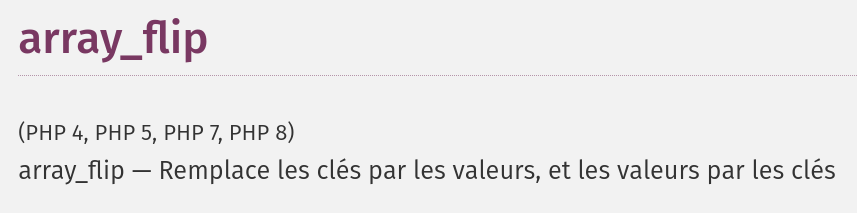
\includegraphics[width=\textwidth]{screenshots/Screenshot_20210526_144450.png}
\end{frame}

\begin{frame}[fragile]{Evaluation paresseuse}{Via un itérateur}
    \begin{lstlisting}[firstnumber=1]
        $output = array_flip(array_flip($input));
    \end{lstlisting}
\end{frame}

\begin{frame}{Schema 0}{Evaluation traditionnelle avec \texttt{array\_flip()}}
    \newcolumntype{t}{>{\tt}c}
        \begin{center}
            \[
            \left[ \begin{array}{tt}
                0 \Rightarrow a \\
                1 \Rightarrow b \\
                2 \Rightarrow c
            \end{array} \right]
            \pause
            \xrightarrow{\texttt{array\_flip()}}
            \left[ \begin{array}{tt}
                a \Rightarrow 0 \\
                b \Rightarrow 1 \\
                c \Rightarrow 2
            \end{array} \right]
            \pause
            \xrightarrow{\texttt{array\_flip()}}
            \left[ \begin{array}{tt}
                0 \Rightarrow a \\
                1 \Rightarrow b \\
                2 \Rightarrow c
            \end{array} \right]
            \]%
    \end{center}
\end{frame}

\begin{frame}{Schema 1}{Evaluation traditionnelle avec \texttt{array\_flip()}}
    \newcolumntype{t}{>{\tt}c}
        \begin{center}
            \[
            \left[ \begin{array}{tt}
                0 \Rightarrow a \\
                1 \Rightarrow b \\
                2 \Rightarrow a
            \end{array} \right]
            \pause
            \xrightarrow{\texttt{array\_flip()}}
            \left[ \begin{array}{tt}
                a \Rightarrow 2 \\
                b \Rightarrow 1
            \end{array} \right]
            \pause
            \xrightarrow{\texttt{array\_flip()}}
            \left[ \begin{array}{tt}
                2 \Rightarrow a \\
                1 \Rightarrow b
            \end{array} \right]
            \]%
    \end{center}
\end{frame}

\begin{frame}{Schema 2}{Evaluation traditionnelle avec \texttt{array\_flip()}}
    \newcolumntype{t}{>{\tt}c}
    \begin{center}
            \[
            \left[ \begin{array}{tt}
                0 \Rightarrow \left[ \begin{array}{tt} a \Rightarrow A\end{array} \right] \\
                1 \Rightarrow \left[ \begin{array}{tt} b \Rightarrow B\end{array} \right] \\
                2 \Rightarrow \left[ \begin{array}{tt} c \Rightarrow C\end{array} \right]
            \end{array} \right]
            \pause
            \xrightarrow{\texttt{array\_flip()}}
            \raisebox{-.5\height}{
\includegraphics[scale=0.05]{meme/No-RageFace.jpg}}
            \]%
            \texttt{Fatal error: Uncaught TypeError: Illegal offset type}
    \end{center}
\end{frame}

\begin{frame}{Schematisons}{evaluation \textit{lazy}}
    \newcolumntype{t}{>{\tt}c}
    \begin{center}
        \[
            \left[ \begin{array}{tt}
                0 \Rightarrow a \\
                1 \Rightarrow b \\
                2 \Rightarrow a
            \end{array} \right]
            \pause
            \xrightarrow{\texttt{array\_flip()}}
            \left[ \begin{array}{tt}
                \only<2->{a \Rightarrow 0} \\
                \only<4->{b \Rightarrow 1} \\
                \only<6->{a \Rightarrow 2}
            \end{array} \right]
            \pause
            \xrightarrow{\texttt{array\_flip()}}
            \left[ \begin{array}{tt}
                \only<3->{0 \Rightarrow a} \\
                \only<5->{1 \Rightarrow b} \\
                \only<7->{2 \Rightarrow a}
            \end{array} \right]
        \]
    \end{center}
\end{frame}

\begin{frame}{Schematisons}{evaluation \textit{lazy}}
    \newcolumntype{t}{>{\tt}c}
    \begin{center}
        \begin{minipage}[adjusting]{.65\textwidth}
            \begin{math}
                \left[ \begin{array}{tt}
                    0 \Rightarrow \left[ \begin{array}{tt} a \Rightarrow A\end{array} \right] \\
                    1 \Rightarrow \left[ \begin{array}{tt} b \Rightarrow B\end{array} \right] \\
                    2 \Rightarrow \left[ \begin{array}{tt} c \Rightarrow C\end{array} \right]
                \end{array} \right]
                \pause
                \xrightarrow{\texttt{array\_flip()}}\newline
                \left[ \begin{array}{tt}
                    \only<2->{\left[ \begin{array}{tt} a \Rightarrow A\end{array} \right] \Rightarrow 0} \\
                    \only<4->{\left[ \begin{array}{tt} b \Rightarrow B\end{array} \right] \Rightarrow 1} \\
                    \only<6->{\left[ \begin{array}{tt} c \Rightarrow C\end{array} \right] \Rightarrow 2}
                \end{array} \right]
                \pause
                \xrightarrow{\texttt{array\_flip()}}\newline
                \left[ \begin{array}{tt}
                    \only<3->{0 \Rightarrow \left[ \begin{array}{tt} a \Rightarrow A\end{array} \right]} \\
                    \only<5->{1 \Rightarrow \left[ \begin{array}{tt} b \Rightarrow B\end{array} \right]} \\
                    \only<7->{2 \Rightarrow \left[ \begin{array}{tt} c \Rightarrow C\end{array} \right]}
                \end{array} \right]
            \end{math}
        \end{minipage}
    \end{center}
\end{frame}


\begin{frame}[fragile]{Evaluation paresseuse}{Juste pour les curieux\ldots \texttt{array\_flip()} paresseux}
    \begin{lstlisting}[firstnumber=1]
        <?php

        function lazy_array_flip(iterable $data): Generator
        {
            foreach ($data as $key => $value) {
                yield $value => $key;
            }
        }

        $input = [
            0 => 'a',
            1 => 'b',
            2 => 'a',
        ];

        $output = iterator_to_array(
            lazy_array_flip(
                lazy_array_flip($input)
            )
        );

        assert($input === $output);
    \end{lstlisting}
\end{frame}

\begin{frameC}{On récapitule\ldots}

\end{frameC}

\begin{frame}{Evaluation paresseuse}{Les \textit{itérateurs et générateurs}, récap}
    \begin{itemize}[<+->]
        \item Par défaut paresseux

        \item Permet d'itérer sur une collection

        \item Permet de dissocier les clés et les valeurs

        \item Permet de corriger les incohérences précitées

        \item A utiliser en connaissance de cause
    \end{itemize}
\end{frame}
